\chapter{Analysis}

\section{Datasets}
In this study, two distinct datasets have been utilized to create a feature table for machine learning algorithms. These datasets are products of Monte Carlo simulations, generated via the SNiPER software, and are essential for understanding the complex physical phenomena under investigation.

\subsection*{IBD Dataset}
The first dataset is designed for analyzing Inverse Beta Decay events and employs temporal ordering and parallel computation with Simulation Identifiers (SimIDs). Parallel computation is vital for efficiently simulating numerous events, though each simulation is independent, resetting t, SimIDs, and other quantities, which is essential for subsequent feature engineering.

In this dataset, each event is simulated, injected, and tagged with a unique SimID. For example, a prompt-delayed pair from an IBD event shares the same SimID. Events triggering enough Photomultiplier Tubes (PMTs) receive an EventID, distinguishing correlated IBD events from uncorrelated ones.

There are cases where electronic noise inadvertently triggers PMTs. These events, saved due to surpassing the trigger threshold, have an EventID but lack a SimID as they aren't injected into the simulation.

The IBD dataset contains \texttt{SimID}, \texttt{EventID}, reconstructed coordinates \texttt{(X, Y, Z)}, energy \texttt{E}, and recording time \texttt{t}.

\subsection*{BKG Dataset}

The second dataset primarily focuses on radioactivity events. This dataset encompasses a large number of simulated events, reflecting the complex reality of real-world physics phenomena. Unlike the IBD dataset, SimID and EventID are not required for the BKG dataset.

One of the key aspects of this dataset is that it accurately accounts for the inherent electronic noise prevalent in actual physical environments, ensuring a realistic representation within the simulated context. The dataset includes events generated from various isotopes and decay rates, as shown in the provided table below:

\begin{table}[htp]
	\centering
	\small
	\begin{tabular}{ccc}
		\toprule
		\textbf{Dataset Name}  & \textbf{Number of Events}  & \textbf{Rates}   \\\midrule
		U238@LS      &   1,000,000 events    &           3.234 Hz            \\
		Th232@LS      &   1,000,000 events    &           0.733 Hz            \\
		K40@LS       &   1,000,000 events    &           0.53 Hz             \\
		Pb210@LS      &   1,000,000 events    &           17.04 Hz            \\
		C14@LS       & 1,000,000,000 events  &           3.3e4 Hz            \\
		Kr85@LS      &   1,000,000 events    &           1.163 Hz            \\
		U238@Acrylic    &   10,000,000 events   &           98.41 Hz            \\
		Th232@Acrylic   &   10,000,000 events   &           22.29 Hz            \\
		
		
		K40@Acrylic    &   10,000,000 events   &          161.25 Hz            \\
		U238@node/bar   &  100,000,000 events   &          2102.36 Hz           \\
		Th232@node/bar   &  100,000,000 events   &          1428.57 Hz           \\
		K40@node/bar    &  100,000,000 events   &           344.5 Hz            \\
		Co60@node/bar   &  100,000,000 events   &           97.5 Hz             \\
		U238@PMTGlass   & 1,000,000,000 events  &          4.90e6 Hz            \\
		Th232@PMTGlass   & 1,000,000,000 events  &          8.64e5 Hz            \\
		K40@PMTGlass    & 1,000,000,000 events  &          4.44e5 Hz            \\
		Tl208@PMTGlass   & 1,000,000,000 events  &          1.39e5 Hz            \\
		Co60@Truss     &           0           &             ? Hz              \\
		Tl208@Truss    &           0           &             ? Hz              \\
		Rn222@WaterRadon  &  100,000,000 events   &            90 Hz              \\
		\bottomrule
	\end{tabular}
	\caption{Table of isotopes and decay rates used in the BKG dataset}
	\label{tab:BKG_gen}
\end{table}


The table showcases the extensive and thorough simulation process. It comprises a rich selection of isotopes, highlighting the intricate nature of radioactivity events.

Focusing on some of the specific entries in the table, U238@PMTGlass has one of the highest decay rates, at approximately 4.90 million Hz. This high rate indicates that Uranium-238 within the PMT Glass is highly active and undergoes decay at a very rapid pace. Such high activity could be significant in the context of the study, as it may contribute substantially to the background noise or signals within the detector.

Similarly, Th232@PMTGlass also exhibits a high decay rate, around 864,000 Hz. Like Uranium-238, Thorium-232 in the PMT Glass is highly active. The high activity levels of these isotopes in the PMT Glass are indicative of the importance of accounting for background signals originating from the detector components themselves.

Another isotope with a high number of events is C14@LS, with a decay rate of approximately 33,000 Hz. While not as high as the rates for isotopes in the PMT Glass, this is still significant and indicates that Carbon-14 in the Liquid Scintillator is also an active contributor to the events being studied.

The diversity in decay rates and the sheer scale of events, especially from isotopes with high decay rates, underscore the complexity of the physical environment being simulated. 

However, not all generated events interact with the detector, and even among those that do, not all are reconstructed. Some events are too low in energy to illuminate the PMTs sufficiently to trigger the acquisition of the event.

%TODO-> Mention unbalanced datasets problem

\newpage

\section{Feature creation}
%TODO: devi sppiegare che il codice è satao runnato su cloudveneto che mi semvra tu non l'abbia mai specifiato.

The development of models for the detection of Inverse Beta Decay (IBD) events necessitates a systematic and efficient approach to feature engineering. This process begins with the loading of the two separate datasets discussed above, one for IBDs and one for radioactivity background.

\subsection{IBD dataset}
As we mentioned earlier, an IBD event is characterized by two distinct signals with different energies, positions, and times. The first, known as the prompt signal, is caused by the annihilation of a positron with an electron in the scintillator liquid. This interaction yields a signal with a characteristic energy. The second, the delayed signal, results from the capture of a neutron by the scintillator liquid. This signal occurs with a significant delay, at a different position, and with a different energy compared to the prompt signal.

To create the feature table, all possible pairs of events within the dataset were considered, without repetition. The ascending temporal order in which the features are created is crucial in feature determination. Given a pair $i-j$, and considering that neutron capture occurs temporally subsequent to electron-positron annihilation, the following features were constructed:


\begin{itemize}
	 
	\item $\mathbf{R_{prompt}}$: This feature represents the distance of the prompt signal, calculated as the distance from the origin to the point $(x_i, y_i, z_i)$ in the detector space where the prompt signal occurred.	
	
	\item $\mathbf{R_{delayed}}$: Similar to $R_{prompt}$, this feature represents the distance of the delayed signal, calculated as the distance from the origin to the point $(x_j, y_j, z_j)$ in the detector space where the delayed signal occurred.

	\item $\mathbf{E_{prompt}}$: This feature represents the energy of the prompt signal. It captures the characteristic energy released during the annihilation of a positron with an electron in the scintillator liquid.

	\item $\mathbf{E_{delayed}}$: This feature represents the energy of the delayed signal. It captures the energy released when a neutron is captured by the scintillator liquid. This capture can occur by hydrogen, resulting in a gamma ray with an energy of approximately 2.2 MeV, or by carbon, resulting in gamma rays with combined energies of about 4.95 MeV to 5.12 MeV.

	\item $\mathbf{\Delta t}$: This feature represents the time difference between the two events. It captures the temporal delay between the occurrence of the prompt and delayed signals.

	\item $\mathbf{\Delta R}$: This feature represents the spatial distance between the two events. It captures the spatial separation between the points in the detector space where the prompt and delayed signals occurred.

\end{itemize}
These features encapsulate the temporal and spatial differences between the prompt and delayed signals, as well as their respective energies, providing a comprehensive representation of the unique characteristics of IBD events.


\subsubsection*{Event Labeling}

The first dataset is designed for the analysis of Inverse Beta Decay events, utilizing temporal ordering and parallel computation with Simulation Identifiers (SimIDs). Parallel computation is key for efficiently simulating a large number of events. However, it's important to note that each parallel simulation is independent and starts from scratch, resetting variables such as t, SimIDs, and other quantities to zero at the beginning of each separate computation. This aspect is crucial to consider in the subsequent feature engineering process.

The label is a binary value: a label of 1 signifies a true IBD event, while a label of 0 signifies a BKG event. The assignment of these labels is not arbitrary but is guided by a specific criterion based on the simulation identifier (SimID) associated with each event pair.

The SimID is used as identifier for assigne to each simulated event pair during the generation the label. If a pair of events share the same SimID, it means they were generated as part of the same simulation and thus are considered to represent a true IBD event. In this case, they are assigned a label of 1.

Conversely, if a pair of events do not share the same SimID, it means they were generated as part of different simulations. These events are not correlated and thus are considered to represent BKG events. In this case, they are assigned a label of 0.


\subsubsection*{Efficient Feature Calculation}
Given the large size of the dataset and the computational complexity of feature calculation, a parallel computing approach was adopted to enhance efficiency. The calculation is done on a virtual machine hosted on Cloud Veneto, with 14 cores of CPU. The feature calculation task was divided into multiple sub-tasks that could be executed simultaneously by the different cores of the CPU. This parallelization significantly reduced the total computation time.

To further optimize the computation, a method was implemented to only consider event pairs where the delayed event occurs within a time window of $5*\tau$ from the prompt event. This approach is based on the fact that the time delay between the prompt and delayed events in Inverse Beta Decay typically follows an exponential distribution, a characteristic of radioactive decay processes. While this method significantly reduces the number of potential event pairs, it might exclude about $0.7\%$ of IBD events that occur outside this time window. 

While this percentage is relatively small, it's important to consider the potential impact on the analysis results.

\subsection{Radioactivity dataset}
For the radioactivity dataset, the feature calculation was performed in a manner analogous to the IBD dataset. The key difference is that event pairs from the radioactivity dataset are labeled as BKG events, hence assigned a label of 0.

The distribution of the features are presented in the Graph \ref{fig:hist_features}.
\begin{figure}[h]
	\centering
	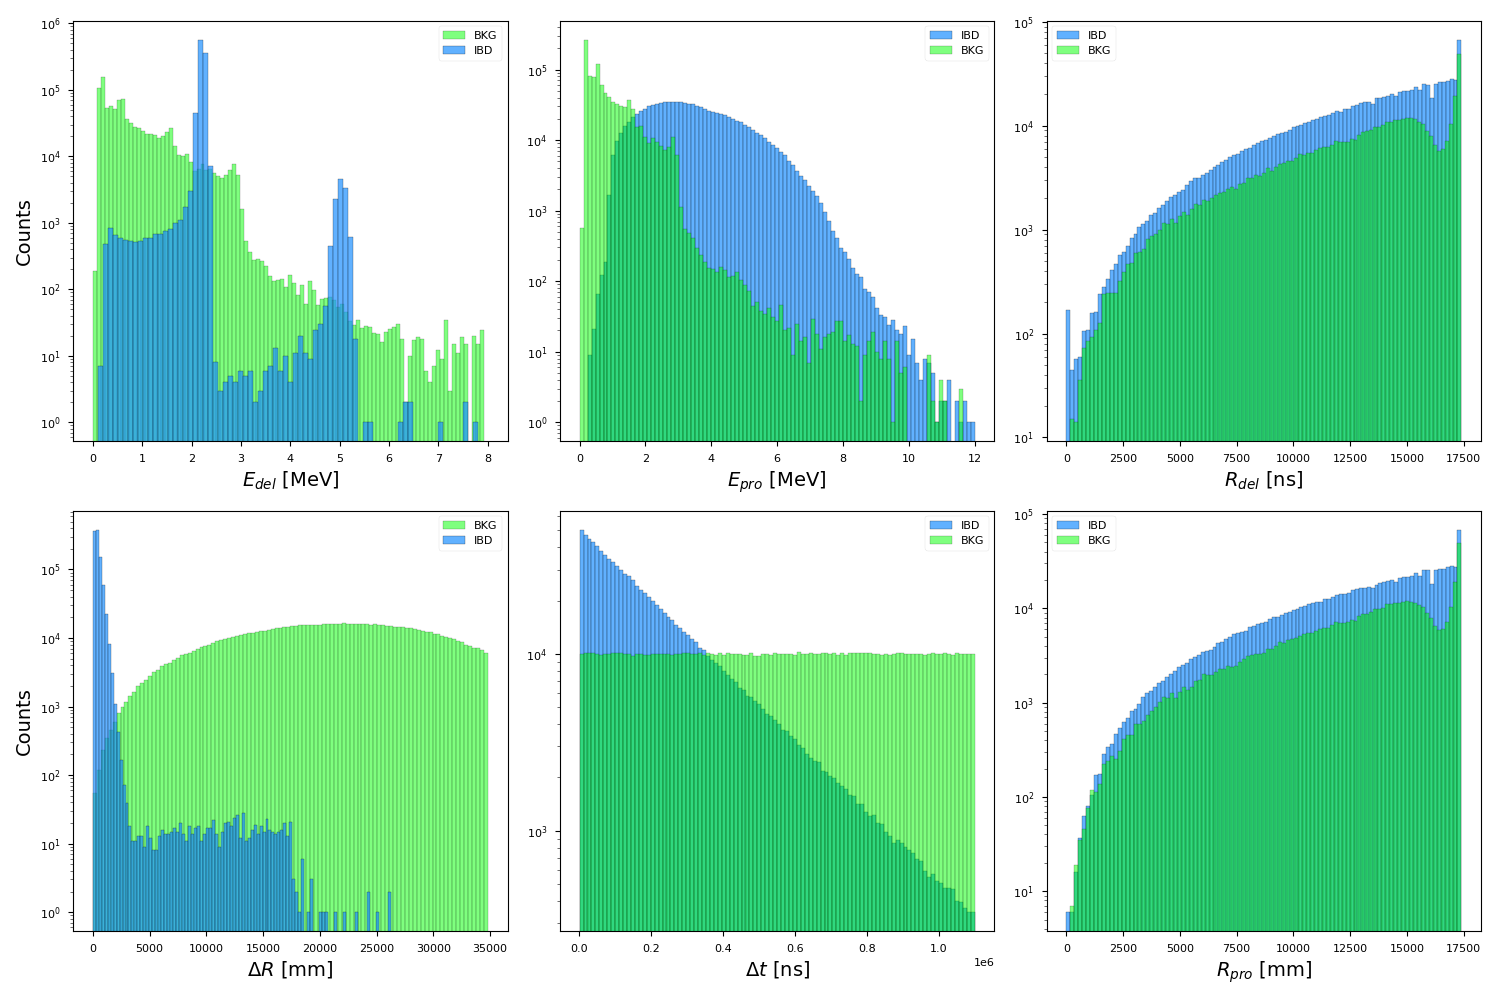
\includegraphics[width=1\linewidth]{Images/hist_features.png}
	\caption{Features histograms}
	\label{fig:hist_features}
\end{figure}

In the presented graph, focusing on $E_{del}$, it is clearly observable the distinct characteristics of the IBD events, such as the peaks at 2.2 MeV and 5.9 MeV, and the clearly visible positron spectrum in the $E_{pro}$. The distribution of $R_{del}$ and $R_{prompt}$ is reasonable, considering the detector's spherical shape, making it more likely for an IBD event to occur in the outer part of the detector due to the greater volume of liquid scintillator. Additionally, the plot for \( \Delta R \) clearly shows that IBD events are generally very close to each other, with a peak observed for \( \Delta R < 3000 \) mm. The \( \Delta t \) distribution for IBD events follows a decreasing exponential distribution, which appears as a straight line since the plot is logarithmic on the y-axis.

For the BKG events, on the other hand, we can see that they have a fundamentally different distribution for \( \Delta R \) compared to IBD events. There is a higher occurrence of events with \( \Delta R > 3000 \) mm, and even at \( \Delta R \approx 35000 \) mm, which corresponds to events occurring in opposite parts of the detector, are significantly probable. This starkly distinguishes IBD events from BKG events. For the \( \Delta t \) distribution of BKG events, it is observed to be nearly constant across all possible \( \Delta t \) values. The number of \( E_{del} \) events decreases as \( E_{del} \) increases, and no well-defined peaks are observed as in the case of IBD events. \( R_{del} \) and \( R_{prompt} \) for BKG events show a distribution similar to IBD events, with the distinction that there are more counts in the final part of the detector, where a higher presence of BKG events is expected due to the surrounding radioactivity activity.


\section{Models}
In the context of the JUNO experiment, a significant part of the effort involves the implementation and optimization of an event selection algorithm. In this chapter, we will present several algorithms for event selection.\\
 
The first one is a manual cut-based approach, \textbf{Manual Cut}, where specific cuts are defined to select events of interest. This approach involves setting criteria based on the physical characteristics of the events and known background noise sources in the detector. The manual cut algorithm allows for precise control over the selection process and enhances the signal-to-background ratio.

In addition to the manual cut algorithm, other algorithms discussed in this chapter are based on machine learning models, specificaly based on \textbf{Boosted Decision Trees} and on \textbf{Neural Network}. 

By exploring both manual cut and machine learning-based algorithms, we aim to provide a comprehensive understanding of different approaches to event selection, highlighting their strengths and limitations in the context of the JUNO experiment.

\subsection{Manual Cut}
The algorithm is designed to suppress various types of background noise while maintaining high efficiency for true IBD events. The selection criteria, or "cuts", are implemented using Python, and are applied to the Features Tables discussed above. Each cut within the algorithm serves a distinct purpose in the overall event selection process.

The key components of the event selection algorithm are as follows:

\begin{enumerate}
	\item \textbf{Delta Time ($\Delta t$) and Delta Radius ($\Delta R$) cuts}: The first cut is applied on the time delay and the radial distance between the prompt and delayed signals. The criteria are:
	\begin{itemize}
		\item Time separation between the prompt and delayed signals should be less than 1.0 ms.
		\item Spatial 3D separation should be less than 1.5 m.
	\end{itemize}

	The specific values in the cuts on Delta Time ($\Delta t$) and Delta Radius ($\Delta R$) are empirically determined based on the characteristics of Inverse Beta Decay events. The 1.0 ms time cut reflects the typical time frame within which the neutron thermalizes and is captured, while the 1.5 m spatial cut accounts for the limited distance that neutrons usually travel before capture. These values are chosen to effectively isolate genuine IBD events by maximizing the signal-to-noise ratio, and are often optimized through simulations and detector response studies.
	
	\vspace{-1\baselineskip}

\begin{figure}[h!]
	\centering
	\begin{minipage}{0.5\textwidth}
		\centering
		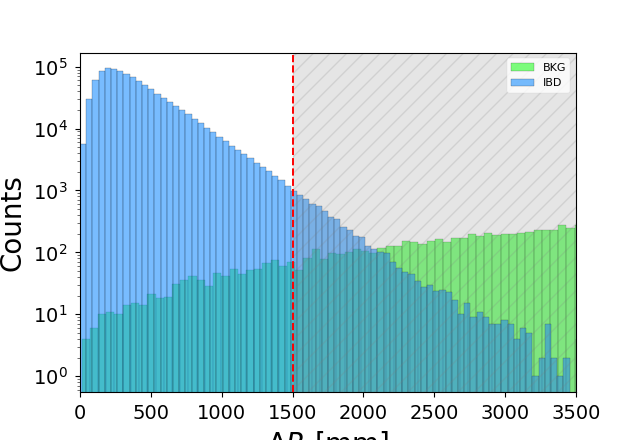
\includegraphics[width=7cm]{Images/Cut/delta_radius.png}
		\caption{$\Delta R$ cut}
		\label{fig:delta_radius_cut}
	\end{minipage}%
	\begin{minipage}{0.5\textwidth}
		\centering
		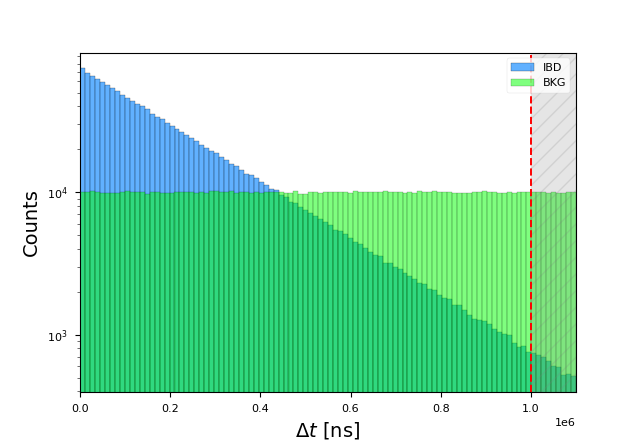
\includegraphics[width=7cm]{Images/Cut/delta_time.png}
		\caption{$\Delta t$ cut}
		\label{fig:delta_t_cut}
	\end{minipage}
\end{figure}


	\vspace{-1\baselineskip}

	\item \textbf{Energy of the Prompt Signal ($E_{pro}$) Cut}: The next cut is applied on the energy of the prompt signal, which is the initial signal produced by the antineutrino interaction. The criteria are:
	\begin{itemize}
		\item Energy of the prompt signal should be within the [0.7, 12.0] MeV range.
	\end{itemize}
	
	\begin{adjustbox}{minipage={\linewidth}, valign=t}
		
		\begin{wrapfigure}{t}{0.5\linewidth}
			
			\vspace{-1\baselineskip}
			\caption{$E_{pro}$ cut}
			\vspace{-0.5\baselineskip}
			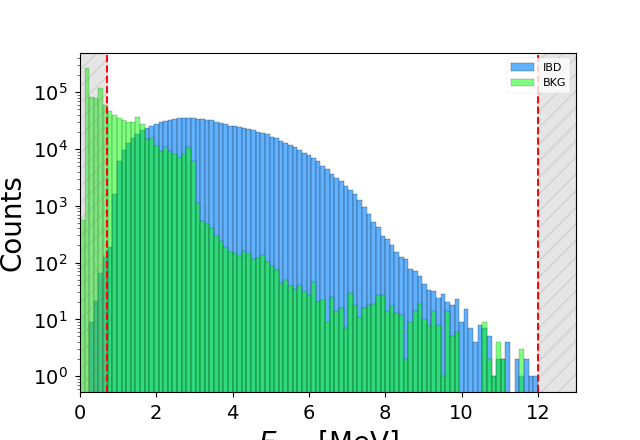
\includegraphics[width=7.5cm]{Images/Cut/e_pro.png}
			\label{fig:e_pto_cut}
			\vspace{-1\baselineskip}
			
		\end{wrapfigure}
		
		\vspace*{0.15cm}
		
		This cut is grounded in the anticipation that the IBD events predominantly occupy this energy range. The energy of the prompt signal is associated with the energy of the positron emanating from the IBD reaction. The selection of this particular range is strategic, aiming to optimize the signal-to-background ratio by focusing on the energy window where IBD events are most likely to occur and where the detector has optimal sensitivity and resolution.
		\\
		
	\end{adjustbox}


	\item \textbf{Energy of the Delayed Signal ($E_{del}$) Cut}: The final cut is applied on the energy of the delayed signal, which is the signal produced by the neutron capture that follows the antineutrino interaction. The criteria are:
	\begin{itemize}
		\item Energy of the delayed signal should be within the [1.9, 2.5] MeV or [4.4, 5.5] MeV ranges.
	\end{itemize}
	
	\begin{adjustbox}{minipage={\linewidth}, valign=t}
		
		\begin{wrapfigure}{t}{0.5\linewidth}
			
			\vspace{-2\baselineskip}
			\caption{$E_{del}$ cut}
			\vspace{-0.5\baselineskip}
			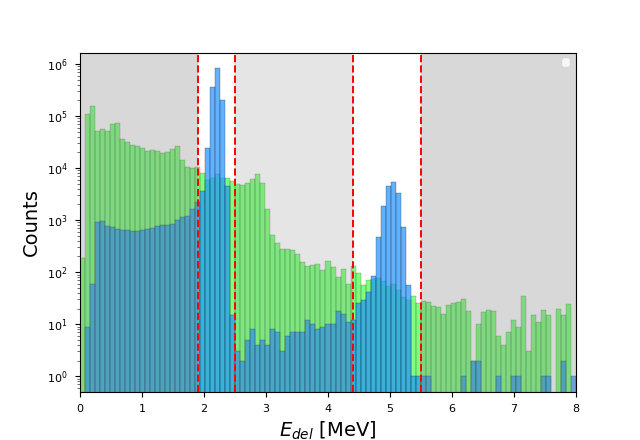
\includegraphics[width=7.5cm]{Images/Cut/e_del.png}
			\label{fig:e_del_cut}
			
		\end{wrapfigure}
		
		\vspace*{0.15cm}
		
		These energy selection windows are aligned with the energies characteristic of neutron capture on hydrogen and carbon atoms. The energy of the delayed signal is a hallmark of the neutron capture process and varies based on the capturing element. The chosen ranges are deliberately selected to coincide with the expected energy signatures for neutron capture on hydrogen and carbon within the detector, which is essential for accurately isolating and analyzing the events of interest.
		\newline
		
	\end{adjustbox}

\end{enumerate}

\subsubsection{Results}
The evaluation showcased the algorithm's adeptness in pinpointing true IBD events and distinguishing them from background noise.

The findings, encompassing the accuracy for true IBD events and efficiency for background events, are organized in two tables. The confusion matrix (Table \ref{tab:confusion_matrix_cut}) offers a comprehensive classification breakdown, while the summary table (Table \ref{tab:performance_cut}) succinctly highlights accuracy rates. The notable efficiency and scarce misclassification of background events underscore the algorithm's prowess in curbing false positives.


\begin{figure}[h!]
	\centering
	\small
	\hspace{-4cm}
	\begin{minipage}{0.3\textwidth}
		\begin{tabular}{cc}
			\toprule
			 & \textbf{Manual Cut} \\ 
			\midrule
			\textbf{IBD Efficiency} &  97.73\% \\ 
			\textbf{BKG Efficiency} &  99.997\% \\ 
			\bottomrule
		\end{tabular}
		\captionof{table}{Performance}
		\label{tab:performance_cut}
	\end{minipage}
\hspace{1.5cm}
	\begin{minipage}{0.5\textwidth}
		\centering
		\begin{tabular}{ccc}
			\toprule
			& \textbf{Predicted IBD} & \textbf{Predicted BKG} \\
			\midrule
			\textbf{Actual IBD} & 1,435,115 & 33,270 \\
			\textbf{Actual BKG} & 26 & 993,457 \\
			\bottomrule
		\end{tabular}
		\captionof{table}{Confusion Matrix}
	\label{tab:confusion_matrix_cut}
	\end{minipage}
	\hspace{-2cm}
\end{figure}

\subsection{XGBoost}
%TODO-> Mention unbalanced datasets problem
%TODO: Cofusion Matrix, Cambiare il max_depth a causa del GridSearch

XGBoost is an optimized gradient-boosting decision tree algorithm, known for its speed and performance, achieved through parallel processing. It's well-suited for complex patterns, making it ideal for the JUNO experiment's event selection.
The XGBoost model was fine-tuned with specific hyperparameters:

\begin{itemize}
	\item  \textbf{Number of parallel threads ($nthread$)} :  Set to -1, utilizing the maximum available threads for faster training.
	\item  \textbf{Random seed ($seed$)} : Set to 1 for reproducibility, ensuring consistent random number generation.
	\item  \textbf{Number of estimators ($n_{estimators}$)} : TConfigured with 10,000 decision trees, controlling model complexity. More trees can improve training performance but may lead to overfitting.
	\item  \textbf{Learning rate ($learning_rate$)} : Set at 0.05, dictating each tree's contribution to the final prediction. A smaller rate makes the model more robust to overfitting.
	\item  \textbf{Maximum tree depth ($max_depth$)} : Limited to 3, controlling the complexity of each tree. A larger depth can lead to overfitting.
\end{itemize}
The chosen hyperparameters strike a balance between computational efficiency and model performance, allowing control over the learning process and model complexity. To optimize the XGBoost model, a Grid Search technique was used. This method systematically evaluated various hyperparameter combinations to identify the optimal configuration that maximizes model accuracy.



\subsubsection{Results}
In this study, the XGBoost algorithm was employed for the classification of true Inverse Beta Decay events. The algorithm exhibited remarkable efficiency in identifying true IBD events and distinguishing them from background events.

A confusion matrix was constructed to provide a comprehensive understanding of the model's precision and effectiveness. The analysis was performed on the total number of IBD and BKG, separately.

The confusion matrix, presented in Table \ref{tab:conf_matrix_xgb}, reveals the number of true positives, false positives, true negatives, and false negatives. The exceptionally low number of false positives and false negatives underscores the algorithm's effectiveness in minimizing misclassifications.

Additionally, the efficiency rates for IBD and background classifications are summarized in a separate table. The high efficiency rates further emphasize the algorithm's proficiency in both identifying true IBD events and rejecting background events.


\begin{figure}[h]
	\centering
	\begin{minipage}{0.33\textwidth}
	\centering
	\begin{tabular}{cc}
		\toprule
		& \textbf{XGBoost} \\
		\midrule
		\textbf{IBD Efficiency} & 99.9972\% \\
		\textbf{BKG Efficiency} & 99.9985\% \\
		\bottomrule
	\end{tabular}
	\captionof{table}{Performance}
	\end{minipage}
	\begin{minipage}{0.65\textwidth}
	\centering
	\begin{tabular}{ccc}
		\toprule
		& \textbf{Predicted IBD} & \textbf{Predicted BKG} \\
		\midrule
		\textbf{Actual IBD} & 1,468,351 & 34 \\
		\textbf{Actual BKG} & 10 & 993,447 \\
		\bottomrule
	\end{tabular}
	\captionof{table}{Confusion Matrix}
	\label{tab:conf_matrix_xgb}
\end{minipage}
\end{figure}




\subsubsection{Interpretation of the model}
In our study, we used \textbf{SHAP} (SHapley Additive exPlanations) to interpret the predictions of a trained XGBoost model. SHAP utilizes concepts from game theory, treating predictions as a "game" where features are the "players". The SHAP value for a feature is its average contribution to every possible combination of features.

The SHAP value, \(\phi_i\), for feature \(i\) is calculated using:

\begin{equation}
	\phi_i = \sum_{S \subseteq N \setminus \{i\}} \frac{|S|!(|N| - |S| - 1)!}{|N|!} [f(S \cup \{i\}) - f(S)]
\end{equation}

Here, \(N\) is the set of all features, \(S\) is a subset of \(N\) excluding feature \(i\), and \(f(S)\) is the model's prediction with feature set \(S\). The term \(\frac{|S|!(|N| - |S| - 1)!}{|N|!}\) assigns a weight to each subset based on the number of times it appears in all permutations of the features.\\



Based on the calculation of SHAP values, we can construct visualizations that aid in analyzing and understanding how the model has learned to differentiate between Inverse Beta Decay events and background events, contributing to model interpretability. 

\begin{figure}[h!]
	\centering
	
	\subfloat[XGBoost Summary Plot]{
		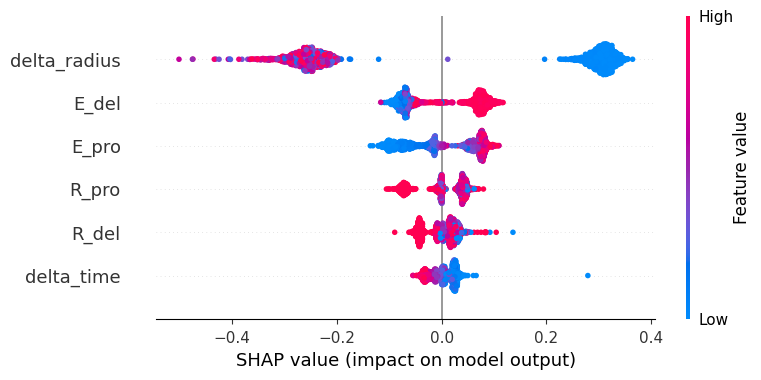
\includegraphics[width = 0.5\textwidth]{Images/Shap/summary_plot.png}
		\label{fig:summary_plot}
	}
	\subfloat[XGBoost feature importance]{
		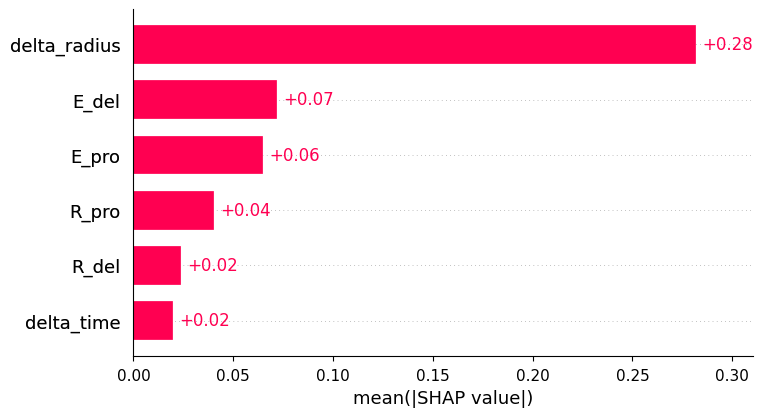
\includegraphics[width = 0.5\textwidth]{Images/Shap/feature_importance_bar.png}
	}
	
\end{figure}


The presented graphs depict the importance of each feature used by the algorithm for learning, measured by calculating the mean of the SHAP values. On the left, we see a histogram where the x-axis represents the mean absolute SHAP value for each feature. The first key characteristic of the model is evident here: the feature with the most importance in classification is $\Delta R$. Moreover, referring back to the Graphs \ref{fig:hist_features}, it was already observable that $\Delta R$ is the feature that separates the IBD class most distinctly from the BKG class. A clear separation is evident from $2500 mm$ onwards, where BKG events prevail, while IBD events are more prevalent below $2500 mm$. The importance of this feature is further highlighted in the right-hand graph, where the x-axis represents the mean absolute SHAP value, and the y-axis represents the various features. Here, the prominence of the feature $\Delta R$ is underscored by the fact that it possesses the highest mean absolute SHAP value, which is 0.28.  \\

Two distinct data clusters for the $\Delta R$ feature are clearly visible. For high values of this feature, the algorithm returns a negative SHAP value, which translates into identification as BKG events, as expected. For lower values of the feature, positive SHAP values are returned, corresponding to events correctly identified as IBD. It's also worth noting that the clusters are perfectly separated, indicating that the algorithm is very confident in labelling events based on this feature.

Second in order of importance, with a SHAP value approximately four times smaller than that of $\Delta R$, is $E_{del}$, the energy of the delayed event. Comparing with the feature histogram, Graph \ref{fig:hist_features}, it's clear that most BKG data occupy the initial part of the histogram, thus at lower energies, and the algorithm has learned to determine that for lower delayed signal energies, the event is classified as a BKG event. For slightly higher energies, given the presence of characteristic peaks that significantly increase the counts of IBD events, the algorithm learns to correctly determine an IBD event. 

Delving deeper into the analysis of this feature, a plot was created where the x-axis represents individual events, and the y-axis represents the effect that each event had on the $E_{del}$ feature. It is observed that for events in the range $\approx[1.9, 2.3] MeV$ and $\approx[4.8, 5.1] MeV$, the algorithm has learned to perfectly distinguish the characteristic peaks of neutron capture compared to all background events.

\begin{figure}[h!]
	\centering
	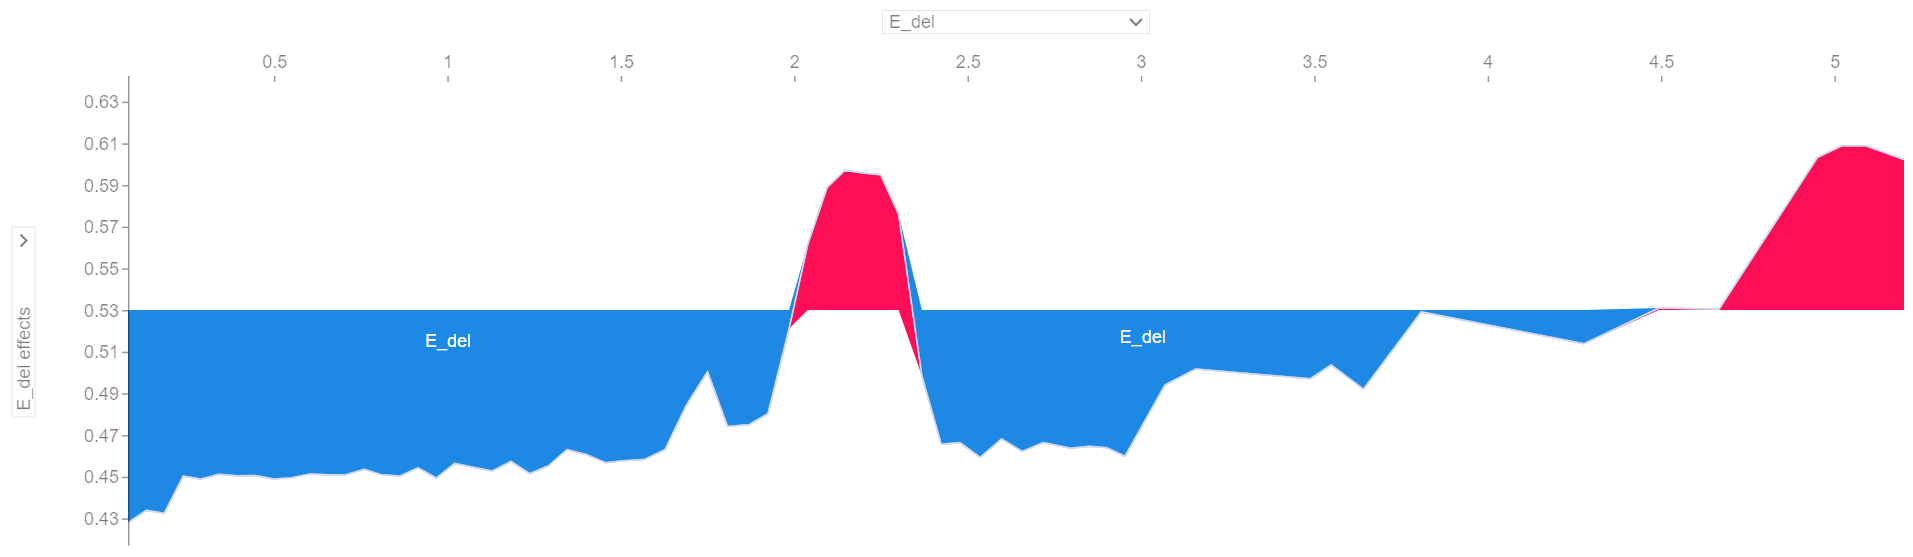
\includegraphics[width=\linewidth]{Images/Shap/E_del_force_plot.png}
	\label{fig:E_del_force_plot}
\end{figure}

Regarding the $E_{pro}$ feature, for values in the range [0, 1] MeV, the histogram is predominantly occupied by BKG events, and as seen from the summary plot, these are correctly identified by the algorithm. However, for prompt signals with energies within the positron-like spectrum, the algorithm identifies these events as IBDs. The features $R_{pro}$, $R_{del}$, and $\Delta t$ do not contribute significantly to the algorithm's ability to discern between the two classes from their distribution, as there are no clear differences between the feature histograms for IBD and BKG.



Based on the aforementioned information, two distinct graphs, known as waterfall plots, are presented. These plots visually display the individual contributions of each feature to the model's final prediction, which is 1 if it's an IBD (Inverse Beta Decay) event and 0 if it's a BKG (background) event. The starting point of these plots is the 'base value', which is calculated as the average of the model's predictions across the entire training dataset. The f(x) shown in the graph represents the predicted value, and is mathematically expressed as:

\begin{equation}
	\text{Final Output} = \text{Base Value} + \sum_{i=1}^{n} \text{SHAP Val}_{i}
\end{equation}

This equation demonstrates how the model arrives at its final prediction by combining the base value with the contributions of each feature through their SHAP values.

\begin{figure}[h!]
	\centering
	\begin{minipage}{0.5\textwidth}
		\centering
		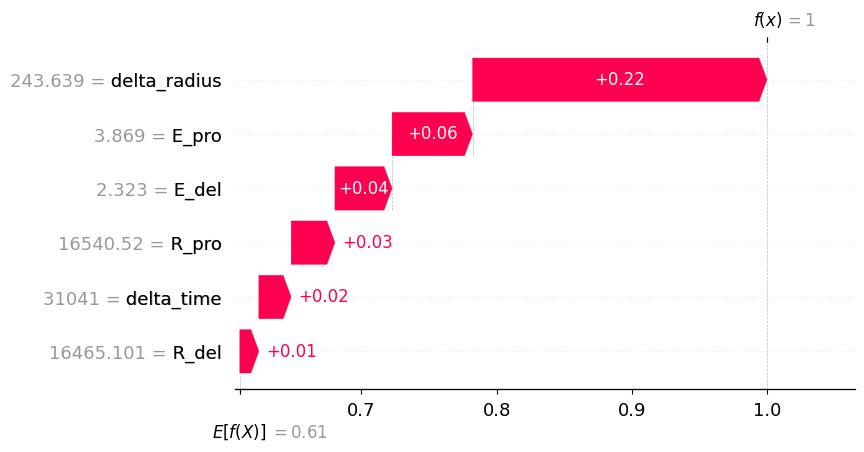
\includegraphics[width=\linewidth]{Images/Shap/waterfall_IBD}
		\caption{Waterfall IBD}
		\label{fig:waterfall_IBD}
	\end{minipage}%
	\begin{minipage}{0.5\textwidth}
		\centering
		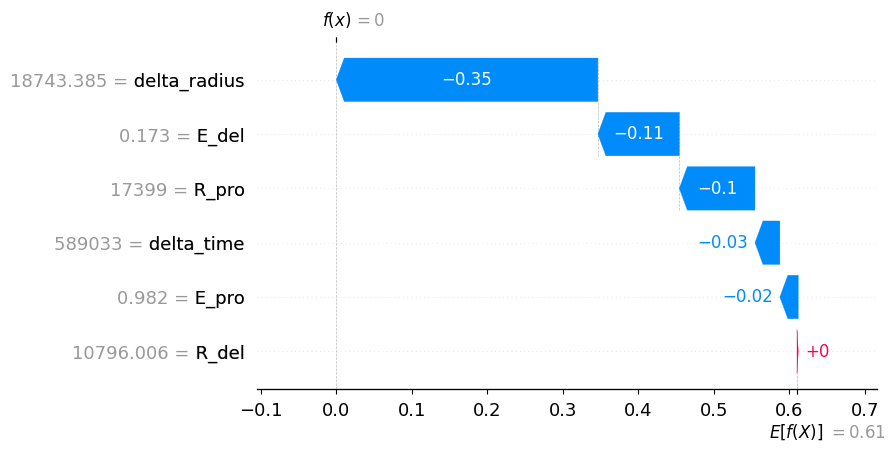
\includegraphics[width=\linewidth]{Images/Shap/waterfall_BKG}
		\caption{Waterfall BKG}
		\label{fig:waterfall_BKG}
	\end{minipage}
\end{figure}

In the SHAP waterfall plots, each feature is represented by a bar, with the length proportional to its SHAP value, indicating its contribution to the prediction. Notably, '\texttt{delta\_radius}' has the longest bar, reflecting its SHAP value of 0.23, for both the predictions, indicating that it is the most influential feature in this instance. Conversely, '\texttt{delta\_time}','\texttt{E\_del}','\texttt{E\_pro}' have the shortest bar due to the SHAP value and the contibution of the prediction, signifying a lesser contribution. This graphical representation provides an intuitive understanding of how each feature is influencing the model's prediction for this particular event, crucial for the interpretability of complex models in neutrino physics.\\
\newline

It is noteworthy to observe how the SHAP values exert influence on the predictions of two mislabeled events, which are, respectively, False Positive and True Negative predictions:


\begin{figure}[h!]
	\centering
	\begin{minipage}{0.5\textwidth}
		\centering
		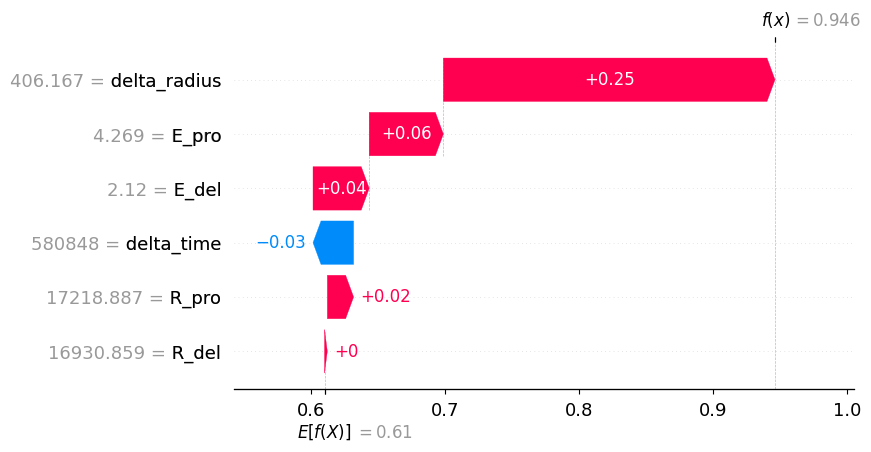
\includegraphics[width=\linewidth]{Images/Shap/waterfall_FP}
		\caption{Waterfall FP}
		\label{fig:waterfall_FP}
	\end{minipage}%
	\begin{minipage}{0.5\textwidth}
		\centering
		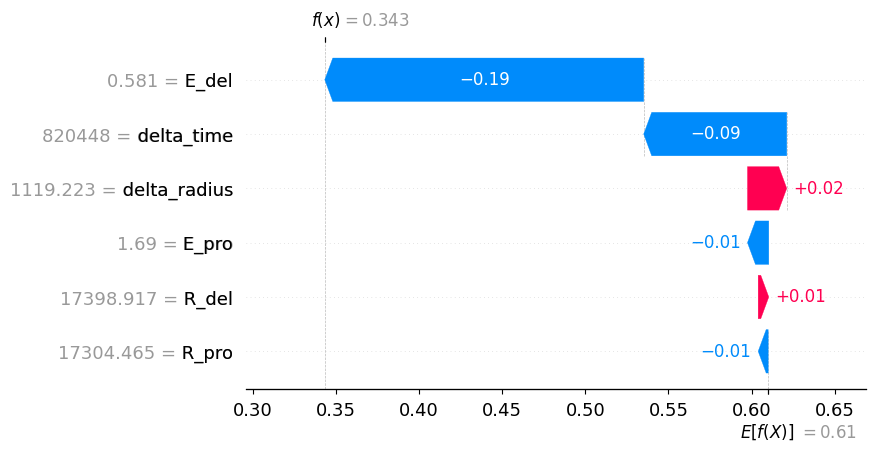
\includegraphics[width=\linewidth]{Images/Shap/waterfall_TN}
		\caption{Waterfall FN}
		\label{fig:waterfall_FN}
	\end{minipage}
\end{figure}


For the \textit{False Negative} case, the most significant feature contributing to the misclassification of the event is $E_{del}$, which is approximately 0.6 MeV. This value does not fall within the characteristic peaks of neutron capture but instead lies in a region where background events (NBKG) are much more probable, as can be compared with Graph \ref{fig:hist_features}. It's important to note that for this particular event, $E_{del}$ is the most influential feature, whereas for most other events, $\Delta R$ (\texttt{delta\_radius}) tends to have a greater contribution. The SHAP value for the $\Delta R$ feature is positive, indicating that this feature suggests the event to be a true IBD, but it is not sufficient for correct labeling. Additionally, the (\texttt{deltatime}) feature contributes to the misclassification because, with a value of approximately 0.8e6 ns, the event falls into a region where background events are more prevalent. The other features are not decisive in the misclassification as they have very small positive and negative SHAP values and do not significantly contribute to correctly identifying the event.

For the \textit{False Positive} case, the feature that contributes the most to the misclassification is $\Delta R$ (\texttt{delta\_radius}). In this case, a coincidence of background events that are very close to each other spatially is misclassified as IBD primarily for this reason, as seen in plot \ref{fig:waterfall_mislab}. Additionally, contributing to the incorrect classification of this event are $E_{del}$ and $E_{pro}$, which have values in regions that are perfectly compatible with the positron spectrum for $E_{pro}$ and compatible with neutron capture for $E_{del}$. Specifically, $E_{del}$ has a value of approximately 2.2 MeV, which is within the expected range for neutron capture.


In conclusion, the SHAP values and the corresponding plots provide a valuable tool for understanding the decision-making process of the model, highlighting the importance of different features in the classification task. 


\subsection{PyThorch}
The ANN, implemented using the PyTorch library, is comprised of one input layer, four hidden layers, and one output layer. The number of neurons in the input layer is determined based on the number of features used in the training dataset, they are ---, so the input layer has 6 input. Each hidden layer contains 64 neurons and utilizes the Rectified Linear Unit (ReLU), $ f(x) = \max(0, x) $, as the activation function. The network eschews an explicit activation function in the output layer and instead produces a direct linear output.

For training the network, it is first instantiated and the computation has been transferred to a CUDA-enabled Graphics Processing Unit (GPU) to leverage hardware acceleration, thereby enhancing computational efficiency. The Cross-Entropy Loss is chosen as the \textit{loss} function due to its efficacy in classification problems. The network's weights are iteratively adjusted through the use of the Adam optimization algorithm.

The training process consists of up to 2000 epochs; however, an early stopping mechanism is integrated to prevent overfitting and to reduce computational overhead. Early stopping functions as an intelligent termination criterion for the training process of a machine learning model. When the model is being trained on a dataset and ceases to exhibit improvement in its performance on an independent validation set, early stopping intervenes to halt the training. This ensures that the model maintains a robust ability to generalize to unseen data and does not overfit by excessively adapting to the idiosyncrasies of the training dataset. 
Specifically, the training is terminated if the validation loss does not exhibit improvement for a span of 10 consecutive epochs.


\subsubsection{Results}


\section{Model Comparison}



\begin{figure}[h!]
	\centering
	\begin{minipage}{0.5\textwidth}
		\centering
		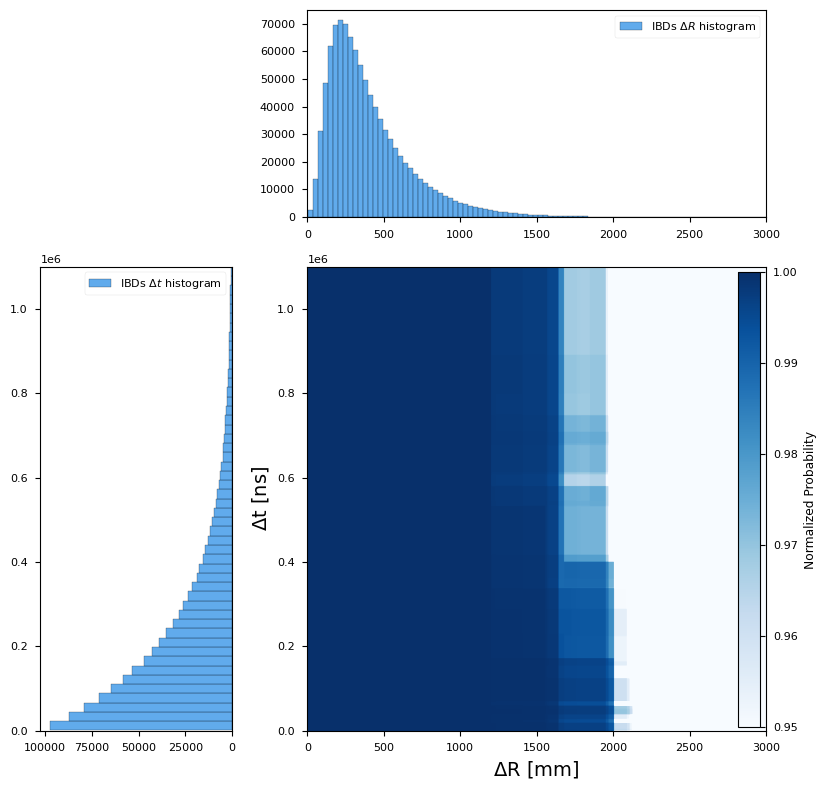
\includegraphics[width=\linewidth]{Images/dr_dt_xgboost}
		\caption{Waterfall FP}
		\label{fig:dr_dt_xgboost}
	\end{minipage}%
	\begin{minipage}{0.5\textwidth}
		\centering
		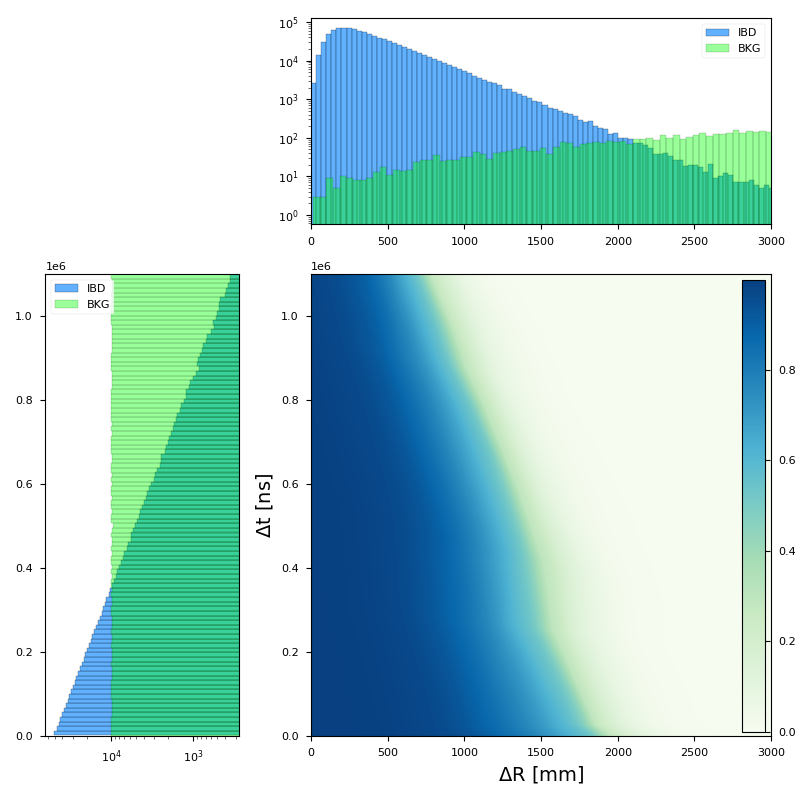
\includegraphics[width=\linewidth]{Images/dr_dt_pytorch}
		\caption{Waterfall FN}
		\label{fig:dr_dt_pytorch}
	\end{minipage}
\end{figure}
The graphs presented illustrate how the two algorithms, XGBoost and PyTorch, evaluate the determination of BKG Ibd events in comparison to BKG events, based on the values of the features $ùDelta R$ and $ùDelta t$. As expected, by observing the distribution of histograms for IBD events only, it is evident that both algorithms perform accurately for events with \texttt{delta\_radius} < 2000mm, identifying IBD events with a probability of at least 97$\%$. The most significant aspect that allows for a comparison between the models through this plot is the feature $delta_t$. Specifically, for XGBoost, as shown in the graph, $delta_t$ does not seem to be very important for determining IBD or BKG events, which is consistent with the feature importance discussed earlier and presented in plot \ref{}. In contrast, for the PyTorch model, the feature $delta_t$ appears to have notable importance for the accurate identification of events. Observing the distribution of the $delta_t$ feature for IBD events reveals an exponential decay, indicating that many IBD events are expected for very low values of $delta_t$, and gradually decreasing. Combining this trend with the decrease in dt events, a graph similar to the one presented for PyTorch is expected. Therefore, even though the PyTorch model has lower efficiency, it seems to better evaluate the importance of the \texttt{delta\_time} feature, which is not achieved with the XGBoost algorithm.

\section{Conclusion}

% Please add the following required packages to your document preamble:
% \usepackage[table,xcdraw]{xcolor}
% If you use beamer only pass "xcolor=table" option, i.e. \documentclass[xcolor=table]{beamer}
\begin{table}[h!]
	\begin{tabular}{lllll}
		\cline{1-3}
		\multicolumn{1}{|l|}{} & \multicolumn{1}{c|}{{\color[HTML]{CE6301} \textbf{Manual Cut Algorithm}}} & \multicolumn{1}{l|}{{\color[HTML]{009901} \textbf{BDT Algorithm}}} &  &  \\ \cline{1-3}
		\multicolumn{1}{|l|}{\textit{Radioactivity}} & \multicolumn{1}{l|}{\begin{tabular}[c]{@{}l@{}}Efficiency: 99.9973\%\\ Purity: 100\%\end{tabular}} & \multicolumn{1}{l|}{\begin{tabular}[c]{@{}l@{}}Efficiency: 99.997684\%\\ Purity: 100\%\end{tabular}} &  &  \\ \cline{1-3}
		\multicolumn{1}{|l|}{\textit{True IBDs}} & \multicolumn{1}{l|}{\begin{tabular}[c]{@{}l@{}}Efficiency: 97.734\%\\ Purity:100\%\end{tabular}} & \multicolumn{1}{l|}{\begin{tabular}[c]{@{}l@{}}Efficiency: 99.997616\%\\ Purity: 100\%\end{tabular}} &  &  \\ \cline{1-3}
		&  &  &  & 
	\end{tabular}
\end{table}

